\begin{center}
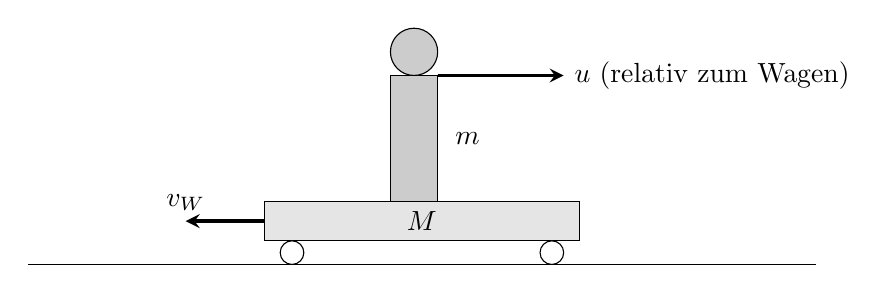
\begin{tikzpicture}[>=stealth]
 \draw (0,0) -- (10,0);
 \draw[fill=gray!20] (3,0.3) rectangle (7,0.8);
 \node at (5,0.55) {$M$};
 \draw[fill=white] (3.35,0.15) circle (0.15) (6.65,0.15) circle (0.15);
 \draw[fill=gray!40] (4.6,0.8) rectangle (5.2,2.4);
 \draw[fill=gray!40] (4.9,2.7) circle (0.3);
 \node[anchor=west] at (5.3,1.6) {$m$};
 \draw[->, very thick] (5.2,2.4) -- (6.8,2.4) node[right] {$u$ (relativ zum Wagen)};
 \draw[->, very thick] (3,0.55) -- (2,0.55) node[above] {$v_\text{W}$};
\end{tikzpicture}
\end{center}

Der Mann geht relativ zum Wagen mit $u = \uReO$ nach rechts, der Wagen fährt mit $v_\text{W} = \vWaO$ nach links. Relativ zum Boden ist der Mann deshalb nur mit
\begin{align}
 v_\text{M} &= \vMaF = \uRe-\vWa = \vMa
\end{align}
unterwegs. Mann und Wagen waren anfänglich in Ruhe, also sind ihre Impulse gleich gross und entgegengesetzt: $m\,v_\text{M} = M\,v_\text{W}$. Damit ist
\begin{align}
 M &= \mWaF \\
   &= \frac{\mMa\cdot\left(\uRe-\vWa\right)}{\vWa} \\
   &= \mWa \approx \result{\mWaP{0}{2}}
\end{align}
